% \section*{Modélisation dynamique d'une structure déformable}

On étudie dans ce problème le comportement d'un objet déformable (poutre 1D) fixé à une extrémité et soumis à l'action d'une force à son autre extrémité. 

On modélise cela par le montage en série de $n$ systèmes ressort-ammortisseur (voir figure \ref{fig1}) présentant, pour tout $0 \leq i < n$, 
%les mêmes masses  $m_i=m$, raideurs $k_i=k $ et coefficients d'amortissement $c_i=c$.
les mêmes masses  $m$, raideurs $k$ et coefficients d'amortissement $c$.
On note $f(t)$ l'intensité de la force appliquée au dernier élément du système. 

% \begin{figure}[!htb]
% \begin{center}
% 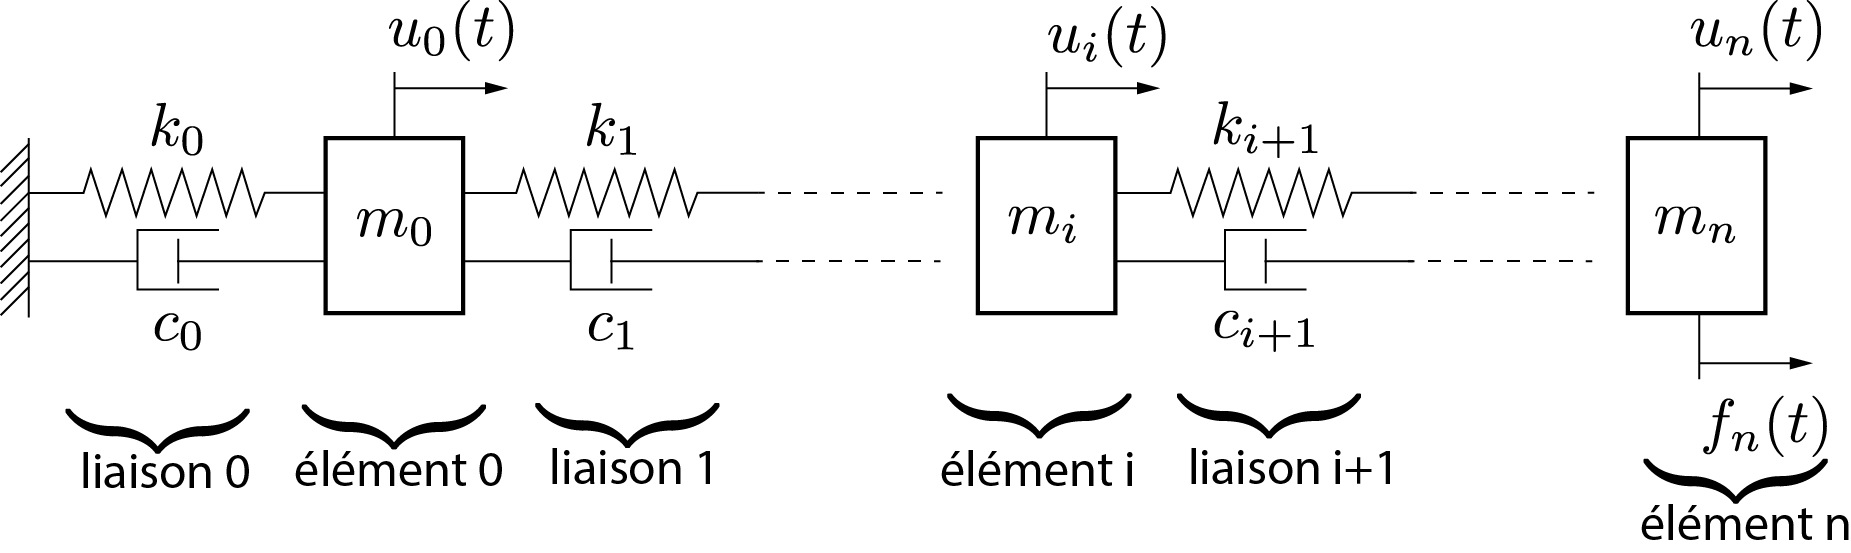
\includegraphics[width=0.9\textwidth]{schemas_ressorts.png}
% \caption{Modélisation de la poutre par un ensemble de masses-ressorts-amortisseurs\label{fig1}}
% \end{center}
% \end{figure}

\begin{figure}[!htb]
\begin{center}
\iflivret
% \documentclass[tikz]{standalone}
% \begin{document}
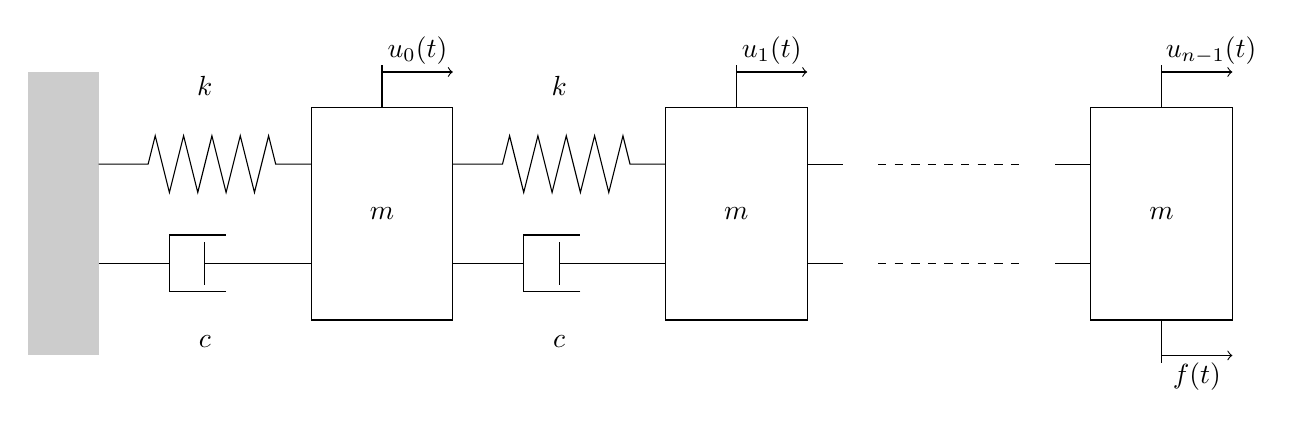
\begin{tikzpicture}[scale=.9]
\fill[black!20] (-1,-2) rectangle (0,2);
\draw (0,.7) -- (.7,.7) -- (.8,1.1) -- (1.0,.3) -- (1.2,1.1) -- (1.4,.3) -- (1.6,1.1) -- (1.8,.3) -- (2.0,1.1) -- (2.2,.3) -- (2.4,1.1) -- (2.5,.7) -- (3.0,.7);
\draw (0,-.7) -- (1,-.7);
\draw (1.8,-1.1) -- (1,-1.1) -- (1,-.3) -- (1.8,-.3); 
\draw (1.5,-1) -- (1.5,-.4);
\draw (1.5,-.7) -- (3,-.7);
\draw (3,-1.5) -- (3,1.5) -- (5,1.5) -- (5,-1.5) -- cycle;
\draw (1.5,-1.8) node  {$c$};
\draw (1.5,1.8) node  {$k$};
\draw (4,0) node {$m$};
\draw (4,1.5) -- (4,2.1);
\draw[->] (4,2) -- (5,2);
\draw (4.5,2.3) node {$u_0(t)$};
\draw (5,.7) -- (5.7,.7) -- (5.8,1.1) -- (6.0,.3) -- (6.2,1.1) -- (6.4,.3) -- (6.6,1.1) -- (6.8,.3) -- (7.0,1.1) -- (7.2,.3) -- (7.4,1.1) -- (7.5,.7) -- (8.0,.7);
\draw (5,-.7) -- (6,-.7);
\draw (6.8,-1.1) -- (6,-1.1) -- (6,-.3) -- (6.8,-.3); 
\draw (6.5,-1) -- (6.5,-.4);
\draw (6.5,-.7) -- (8,-.7);
\draw (8,-1.5) -- (8,1.5) -- (10,1.5) -- (10,-1.5) -- cycle;
\draw (6.5,-1.8) node  {$c$};
\draw (6.5,1.8) node  {$k$};
\draw (9,0) node {$m$};
\draw (9,1.5) -- (9,2.1);
\draw[->] (9,2) -- (10,2);
\draw (9.5,2.3) node {$u_1(t)$};
\draw (10,.7) -- (10.5,.7);
\draw[dashed] (11,.7) -- (13,.7);
\draw (13.5,.7) -- (14,.7);
\draw (10,-.7) -- (10.5,-.7);
\draw[dashed] (11,-.7) -- (13,-.7);
\draw (13.5,-.7) -- (14,-.7);
\draw (14,-1.5) -- (14,1.5) -- (16,1.5) -- (16,-1.5) -- cycle;
\draw (15,0) node {$m$};
\draw (15,1.5) -- (15,2.1);
\draw[->] (15,2) -- (16,2);
\draw (15.7,2.3) node {$u_{n-1}(t)$};
\draw (15,-1.5) -- (15,-2.1);
\draw[->] (15,-2) -- (16,-2);
\draw (15.5,-2.3) node {$f(t)$};
\end{tikzpicture}

% \end{document}
\else
% \documentclass[tikz]{standalone}
% \begin{document}
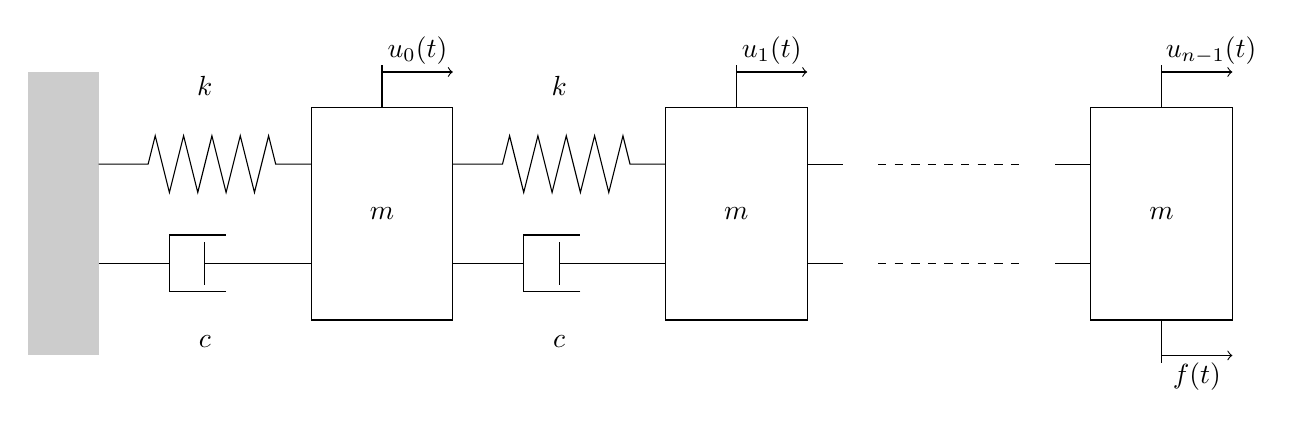
\begin{tikzpicture}[scale=.9]
\fill[black!20] (-1,-2) rectangle (0,2);
\draw (0,.7) -- (.7,.7) -- (.8,1.1) -- (1.0,.3) -- (1.2,1.1) -- (1.4,.3) -- (1.6,1.1) -- (1.8,.3) -- (2.0,1.1) -- (2.2,.3) -- (2.4,1.1) -- (2.5,.7) -- (3.0,.7);
\draw (0,-.7) -- (1,-.7);
\draw (1.8,-1.1) -- (1,-1.1) -- (1,-.3) -- (1.8,-.3); 
\draw (1.5,-1) -- (1.5,-.4);
\draw (1.5,-.7) -- (3,-.7);
\draw (3,-1.5) -- (3,1.5) -- (5,1.5) -- (5,-1.5) -- cycle;
\draw (1.5,-1.8) node  {$c$};
\draw (1.5,1.8) node  {$k$};
\draw (4,0) node {$m$};
\draw (4,1.5) -- (4,2.1);
\draw[->] (4,2) -- (5,2);
\draw (4.5,2.3) node {$u_0(t)$};
\draw (5,.7) -- (5.7,.7) -- (5.8,1.1) -- (6.0,.3) -- (6.2,1.1) -- (6.4,.3) -- (6.6,1.1) -- (6.8,.3) -- (7.0,1.1) -- (7.2,.3) -- (7.4,1.1) -- (7.5,.7) -- (8.0,.7);
\draw (5,-.7) -- (6,-.7);
\draw (6.8,-1.1) -- (6,-1.1) -- (6,-.3) -- (6.8,-.3); 
\draw (6.5,-1) -- (6.5,-.4);
\draw (6.5,-.7) -- (8,-.7);
\draw (8,-1.5) -- (8,1.5) -- (10,1.5) -- (10,-1.5) -- cycle;
\draw (6.5,-1.8) node  {$c$};
\draw (6.5,1.8) node  {$k$};
\draw (9,0) node {$m$};
\draw (9,1.5) -- (9,2.1);
\draw[->] (9,2) -- (10,2);
\draw (9.5,2.3) node {$u_1(t)$};
\draw (10,.7) -- (10.5,.7);
\draw[dashed] (11,.7) -- (13,.7);
\draw (13.5,.7) -- (14,.7);
\draw (10,-.7) -- (10.5,-.7);
\draw[dashed] (11,-.7) -- (13,-.7);
\draw (13.5,-.7) -- (14,-.7);
\draw (14,-1.5) -- (14,1.5) -- (16,1.5) -- (16,-1.5) -- cycle;
\draw (15,0) node {$m$};
\draw (15,1.5) -- (15,2.1);
\draw[->] (15,2) -- (16,2);
\draw (15.7,2.3) node {$u_{n-1}(t)$};
\draw (15,-1.5) -- (15,-2.1);
\draw[->] (15,-2) -- (16,-2);
\draw (15.5,-2.3) node {$f(t)$};
\end{tikzpicture}

% \end{document}
\fi
\end{center}
\caption{Modélisation de la poutre par un ensemble de masses-ressorts-amortisseurs\label{fig1}}
\end{figure}



Pour tout $0 \leq i < n$ et tout temps $t$, on note $u_i(t)$ le déplacement de l'élément \no$i$ par rapport à sa position d'équilibre et l'on introduit le vecteur 
\begin{equation*}
  X(t) = \begin{pmatrix} u_0(t) \\ \vdots \\ u_{n-1}(t) \end{pmatrix}.
\end{equation*}
On peut montrer que $X$ vérifie l'équation différentielle 
\begin{equation*}
  MX'' + CX' + KX = F(t),
\end{equation*}
où
\begin{align*}
  M &= \begin{pmatrix} m & 0  & \cdots&\cdots & 0\\
0 & m  & 0 & \cdots & \vdots\\
\vdots & 0  & \ddots & \ddots & \vdots\\
\vdots & \vdots  &\ddots & m & 0\\
0 & 0  &  \cdots & 0 & m\\ \end{pmatrix}&,
\quad C &= \begin{pmatrix} 2c & -c  & 0&\cdots & 0\\
-c & 2c  & -c & \ddots & \vdots\\
0 & -c  & \ddots & \ddots & 0\\
\vdots & \ddots  &\ddots & 2c & -c\\
0 &  \cdots  &  0 & -c & 2c\\ \end{pmatrix}, \\
K &= \begin{pmatrix} 2k & -k  & 0&\cdots & 0\\
-k & 2k  & -k & \ddots & \vdots\\
0 & -k  & \ddots & \ddots & 0\\
\vdots & \ddots  &\ddots & 2k & -k\\
0 &  \cdots  &  0 & -k & 2k\\ \end{pmatrix}&,
\quad
F(t) &= \begin{pmatrix} 0 \\ \vdots \\ 0 \\ f(t) \end{pmatrix}.
\end{align*}
Les matrices carrées écrites ici sont de dimension $n\times n$ et le vecteur $F(t)$ est de dimension $n$. 

On utilise la méthode d'Euler pour résoudre de manière approchée cette équation différentielle. On fixe donc un pas de temps $\texttt{dt} > 0$ et l'on calcule de proche en proche les 
\begin{equation*}
  X_q = X(q \times \texttt{dt}).
\end{equation*}
Le système est au repos au départ, on suppose donc que $X_0 = X_{-1} = 0$.

Avec
\begin{equation*}
  H = \dfrac{1}{\texttt{dt}^2} M + \dfrac{1}{\texttt{dt}}C + K
\end{equation*}
et, pour tout $q \geq 1$,
\begin{equation*}
  G_q = \dfrac{1}{\texttt{dt}^2} M (2X_{q-1} - X_{q-2}) + \dfrac{1}{\texttt{dt}}CX_{q-1} + F(q\times \texttt{dt}),
\end{equation*}
on montre que, pour tout $q \geq 1$,
\begin{equation*}
  H \times X_q = G_q.
\end{equation*}
On remarquera que, comme les matrices $C$ et $K$, $H$ est tridiagonale. 

Pour mettre en {\oe}uvre la méthode d'Euler, on résout donc plusieurs systèmes de même membre de gauche $H$. Nous allons utiliser ici la méthode de Jacobi pour résoudre ce système.

\medskip{}

\question{} Écrire une fonction \texttt{matrice\_H(m,c,k,dt,n)} prenant en argument quatre flottants strictement positifs \texttt{m}, \texttt{c}, \texttt{k} et \texttt{dt} ainsi qu'un entier strictement positif \texttt{n} et renvoyant la matrice $H$ de dimension $\texttt{n} \times \texttt{n}$ définie ci-dessus.  

\medskip{}

On donne la fonction suivante, permettant de calculer le vecteur $G_q$.
\begin{verbatim}
import numpy as np

def vecteur_G(m,c,dt,q,X1,X2,f):
    """Renvoie le vecteur Gq de dimension n
    Préconditions : m,c,dt flottants strictements positifs
                    q entier positif
                    X1,X2 vecteurs nx1 (X1 : X_q-1 et X2 = X_q-2)
                    f fonction réelle, appel en O(1)"""
    n,_ = X1.shape
    G = np.zeros((n,1))
    for i in range(n):
        G[i] = m*(2X1[i]-X2[i])/(dt**2)
    G[0] = G[0] +  (2c * X1[0] - c*X1[1])/dt
    G[-1] = G[-1] +  (2c * X1[-1] - c*X1[-2])/dt + f(q*dt)
    for i in range(1,n-1) : 
        G[i] = G[i] + (2c * X1[i] - c*X1[i-1] - c*X1[i+1])/dt
    return G
\end{verbatim}


\medskip{}

\question{} Étudier la complexité temporelle d'un appel de la fonction \texttt{vecteur\_G(m,c,dt,q,X1,X2,f)}, en fonction d'une grandeur que l'on explicitera. 

\medskip{}

La méthode du pivot de Gauss étant numériquement peu stable, on lui préfère souvent des méthodes itératives. On expose ici celle de Jacobi. 

\medskip{}

On résout le système $n\times n$ écrit matriciellement : $H\times Y = G$, à partir d'un vecteur initial $Y^0$. 
Pour tout $q \in \N$, on note 
\begin{equation*}
  Y^q = \begin{pmatrix} y^q_0 \\ \vdots \\ y^q_{n-1} \end{pmatrix}.
\end{equation*}


Si le vecteur $Y^q$ est construit, la méthode de Jacobi consiste à définir le vecteur $Y^{q+1}$ par, pour tout $0 \leq i < n$,
\begin{equation*}
  y^{q+1}_i = \dfrac{1}{h_{i,i}} \left(g_i - \sum_{j\neq i} h_{i,j} y^q_j\right).
\end{equation*}

\medskip{}

\question{} Proposer une simplification de la somme écrite ci-dessus utilisant le fait que la matrice $H$ utilisée ici est tridiagonale (on distinguera les cas $i=0$ et $i=n-1$).

\medskip{}

\question{} Écrire une fonction \texttt{iteration\_Jacobi(H,G,Yq)} prenant en argument une matrice $H$ tridiagonale ainsi que deux vecteurs \texttt{G} et \texttt{Yq}, renvoie le vecteur $Y^{q+1}$ décrit ci-dessus.

\emph{On s'interdira ici d'utiliser la multiplication matricielle fournie par la bibliothèque \texttt{numpy}}.

\medskip{}

On considère la norme euclidienne d'un vecteur : 
\begin{equation*}
  \norm{\begin{pmatrix} x_0 \\ \vdots \\ x_{n-1} \end{pmatrix}} = \sqrt{x_0^2 + \dots + x_{n-1}^2} = \sqrt{\sum_{k=0}^{n-1}x_k^2}.
\end{equation*}

\medskip{}

\question{} Écrire une fonction \texttt{carre\_norme(X)} prenant en argument un vecteur \texttt{X} et renvoyant le carré de sa norme, \emph{i.e.} $\norm{X}^2$.

\medskip{}

On utilise le critère d'arrêt suivant pour la méthode de Jacobi : on fixe une précision $\eps>0$, on s'arrête dès que $\norm{HY_q - G} \leq \eps \norm{G}$ et l'on prend $Y_q$ comme approximation de la solution de ce système.

\medskip{}

\question{} Écrire une fonction \texttt{Jacobi(H,G,Y0,eps)} prenant en argument une matrice tridiagonale \texttt{H}, deux vecteurs \texttt{G} et \texttt{Y0} ainsi qu'un flottant strictement positif \texttt{eps} et renvoyant la valeur approchée du système $\texttt{H} \times X = \texttt{G}$ avec la condition initiale \texttt{Y0} et le critère d'arrêt donné par $\eps = \texttt{eps}$.

\medskip{}

La méthode de Jacobi converge si la matrice $H$ est à diagonale strictement dominante, \emph{i.e.} si pour tout $0 \leq i < n$, 
\begin{equation*}
  \abs{h_{i,i}} > \sum_{j\neq i} \abs{h_{i,j}}.
\end{equation*}

\medskip{}

\question{} Justifier que la méthode de Jacobi est ici convergente.

\medskip{}

\emph{N'attaquez la dernière question que si vous avez traité toutes les autres questions correctement.}

\question{} On effectue ce calcul sur $p$ valeurs de temps distinctes. On rappelle que l'on résout donc $p$ systèmes de la forme $H \times X_q = G_q$. Toujours en utilisant la méthode de Jacobi, peut-il être préférable de mettre en {\oe}uvre une autre stratégie de résolution, du point de vue de la complexité temporelle ?

\emph{On pourra supposer que tous les appels de la fonction \texttt{Jacobi} ont la même complexité temporelle.}